\section {Systematic Uncertainties on the Search}

The source of systematic uncertainties are considered as following:
\begin{itemize}
\item Jet Energy Scale (JES)
\item Jet Energy Resolution (JER) 
\item Choise of Background Parametrization
\item Luminosity
\end{itemize}
Our procedure to evaluate the first three is to use a smooth fit to the 
QCD background as a data sample, and find the cross section upper limits for 
this data sample before and after systematic shifts, described below. 

\subsection{Jet Energy Scale (JES)} 
The uncertainty on the JES that is important for this analysis
is the uncertainty on how well the dijet resonance simulation models the jet energy scale of real jets.
If the simulation produces jets with too high a response, then the true position of the expected resonance
peak for that resonance mass would really be at lower mass than predicted by the simulation.
We assume that the uncertainty on JES is roughly $\pm10\%$ and test the sensitivity of our 
analysis to a shift in the resonance signal by 10\%. Shifting the resonance 10\% lower in dijet mass 
gives more background from QCD and finding the resonance signal is harder.\\
The left plot in Fig.~\ref{JES} shows smooth cross section limit without systematics and with systematics on JES uncertainty for $qg$ resonance. 
To get smooth cross section limit curve, expected events from background, $N_{i}(B)$, which is smooth and comes from fit function are considered 
as measurement number of events, $n_{i}$, in the $i-th$ dijet mass bin. 
Fractional change between smooth limits are illustrated separately at right plot of Fig.~\ref{JES}. The 
systematic uncertainty decreases with resonance mass primarily because we are setting limits at the
edge of the region with real data, and the uncertainty is very sensitive to whether any data events are
expected from the background: if there is no background, there is no change in the limit with JES uncertainty.
This systematic has increased with luminosity at high resonance mass, and we expect that this systematic 
uncertainty will continue to increase as we get more data.

\begin{figure}[!ht]
  \begin{center}
%   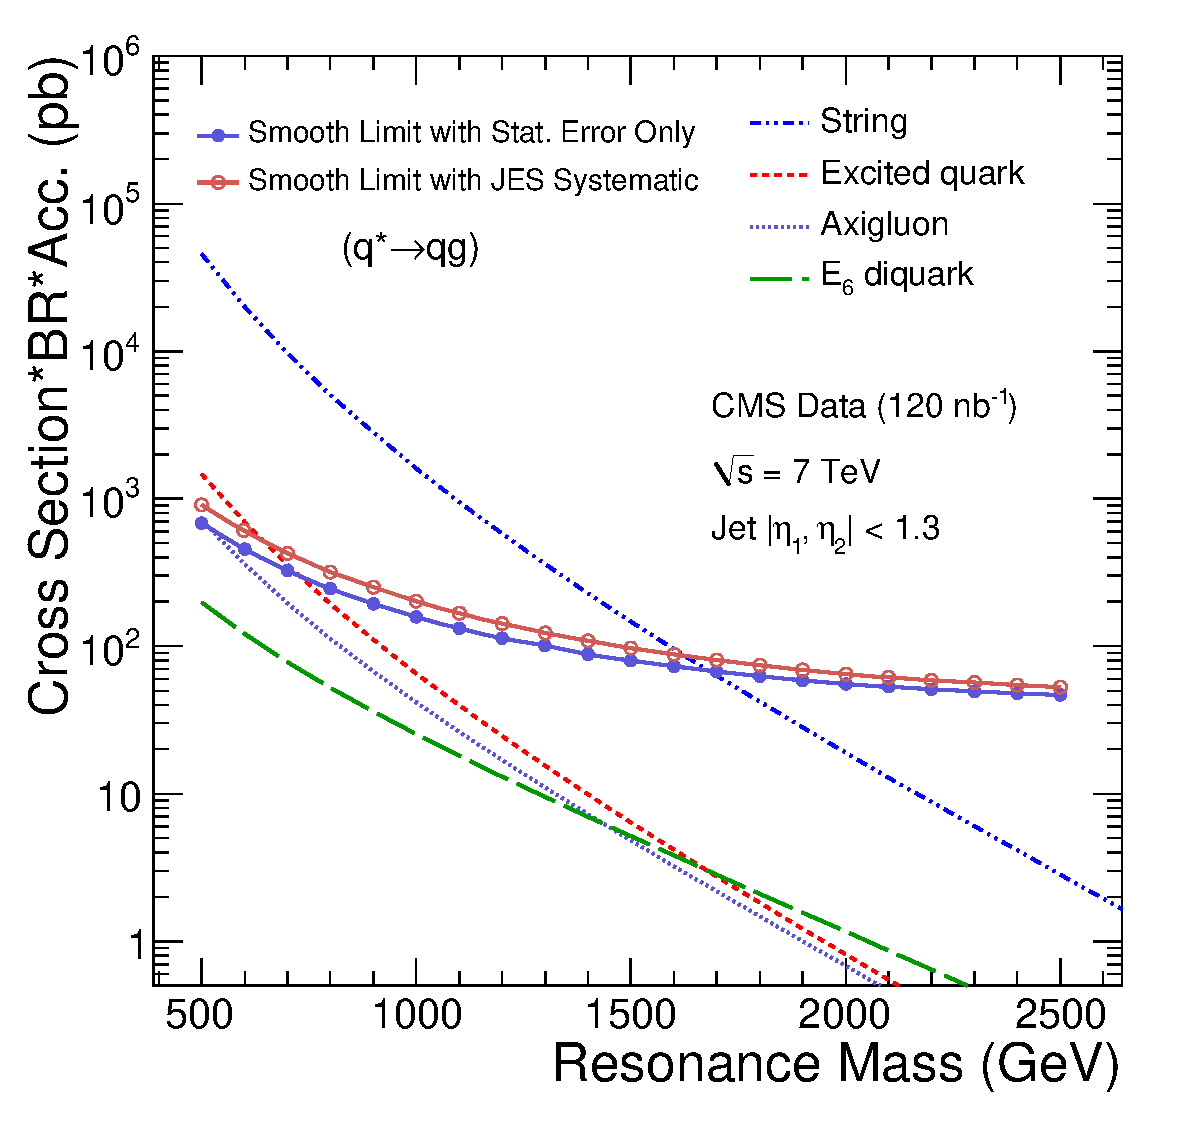
\includegraphics[width=0.45\textwidth]{Figures/Limit_Comparison_JES_Systematic.pdf}
   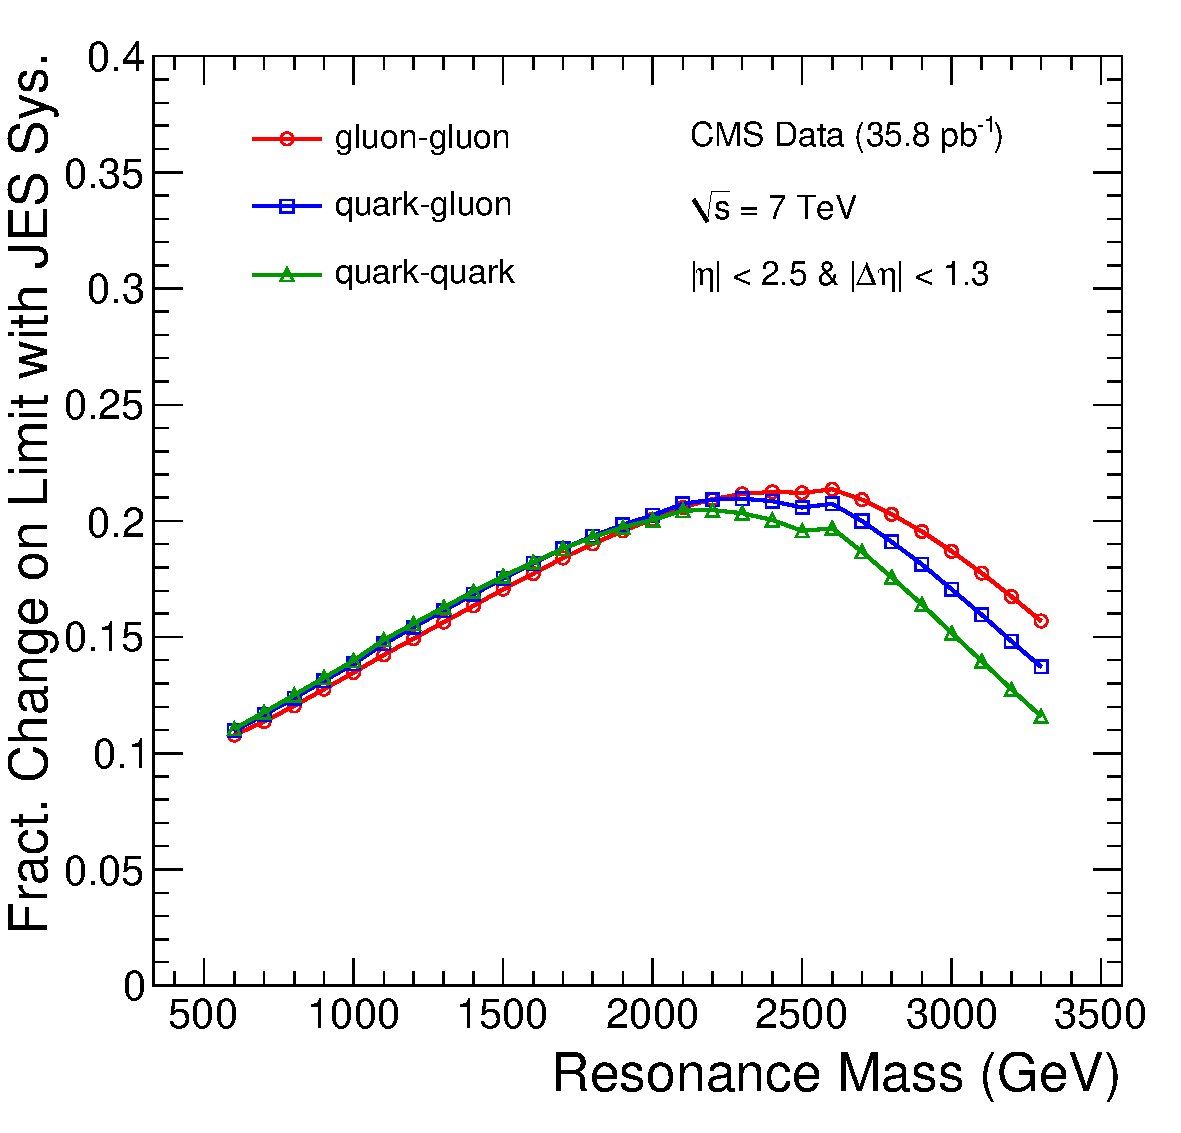
\includegraphics[width=0.45\textwidth]{Figures/Fractional_Change_JES_All.pdf}
    \caption{ 
%\textit{Left plot}: Comparison of smoothed cross section limit with and without JES systematic uncertainty.
%\textit{Right plot}:
Fractional change on limit with JES systematic uncertainty.}
    \label{JES}
  \end{center}
\end{figure}
\clearpage

\subsection{Jet Energy Resolution (JER)}

JetMET recommends a resolution systematic of 10\% which is supported by the first measurements
of the RMS resolution in data using the dijet $p_T$ asymmetry method~\cite{PAS_JME_10-003}.
The tails of the resolution function are in good agreement between data and MC~\cite{CMS_AN_2010/134}.
This same dijet asymmetry method with a varying cut on the 3rd jet pt constrains the differences in 
radiation between the data and MC~\cite{CMS_AN_2010/134}, and thereby constrains differences in MC 
modelling of the resonance shape due to radiation to not be a big effect.
We assume that the uncertainty on JER is roughly $\pm10\%$ and the signal is being smeared 
with a Gaussian that increases the core resolution by 10\%. A comparison of resonace shapes are shown in
Fig.\ref{conv_shape}.

\begin{figure}[!ht]
  \begin{center}
     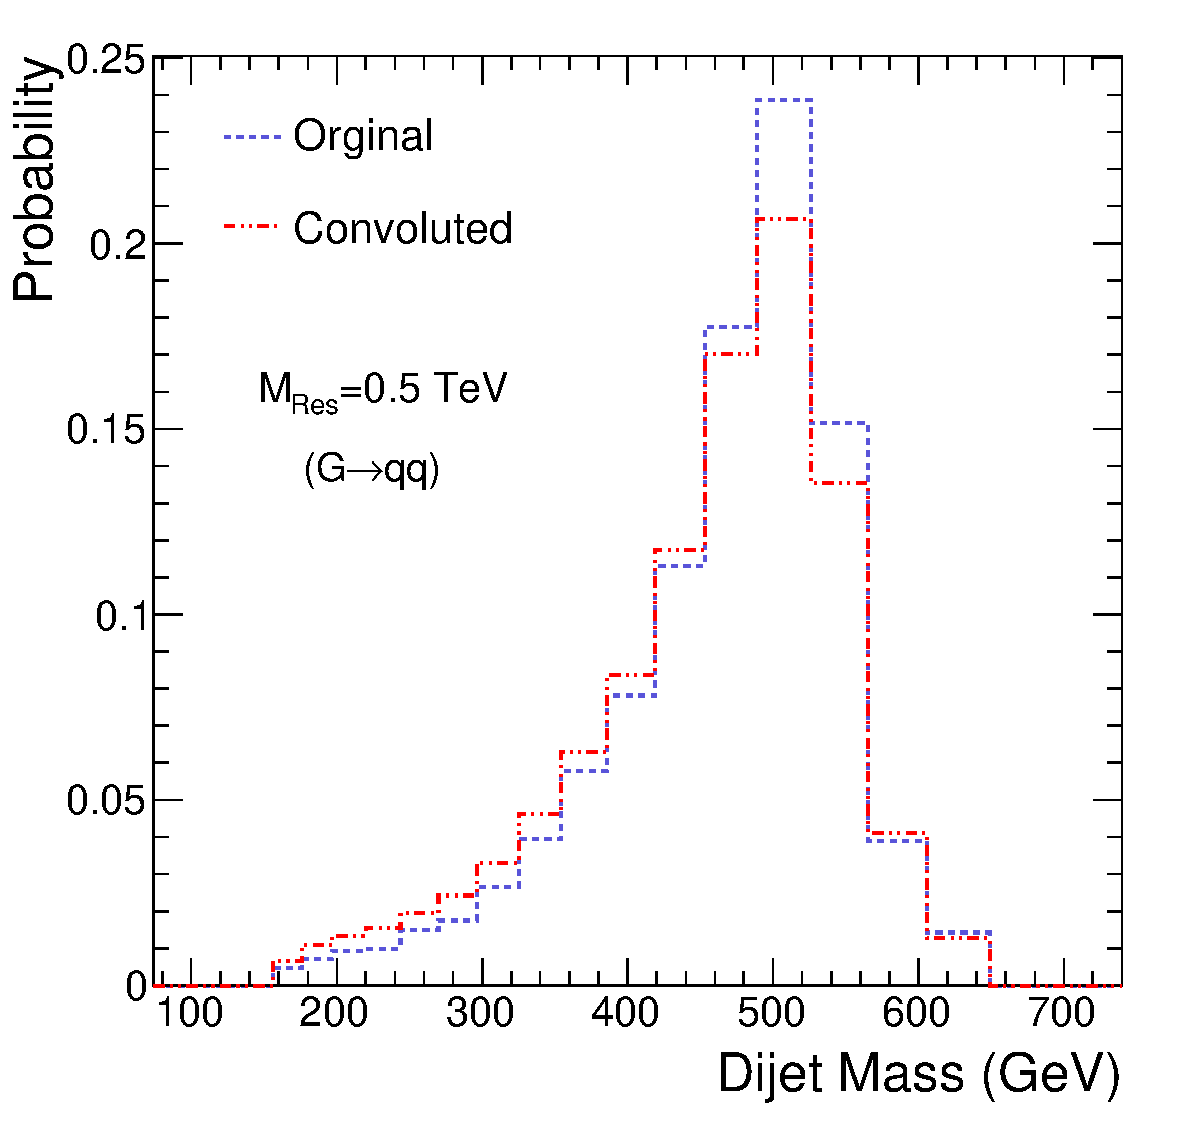
\includegraphics[width=0.3\textwidth]{Figures/Resonace_Shape_Convoluted_qq_1200.pdf}
       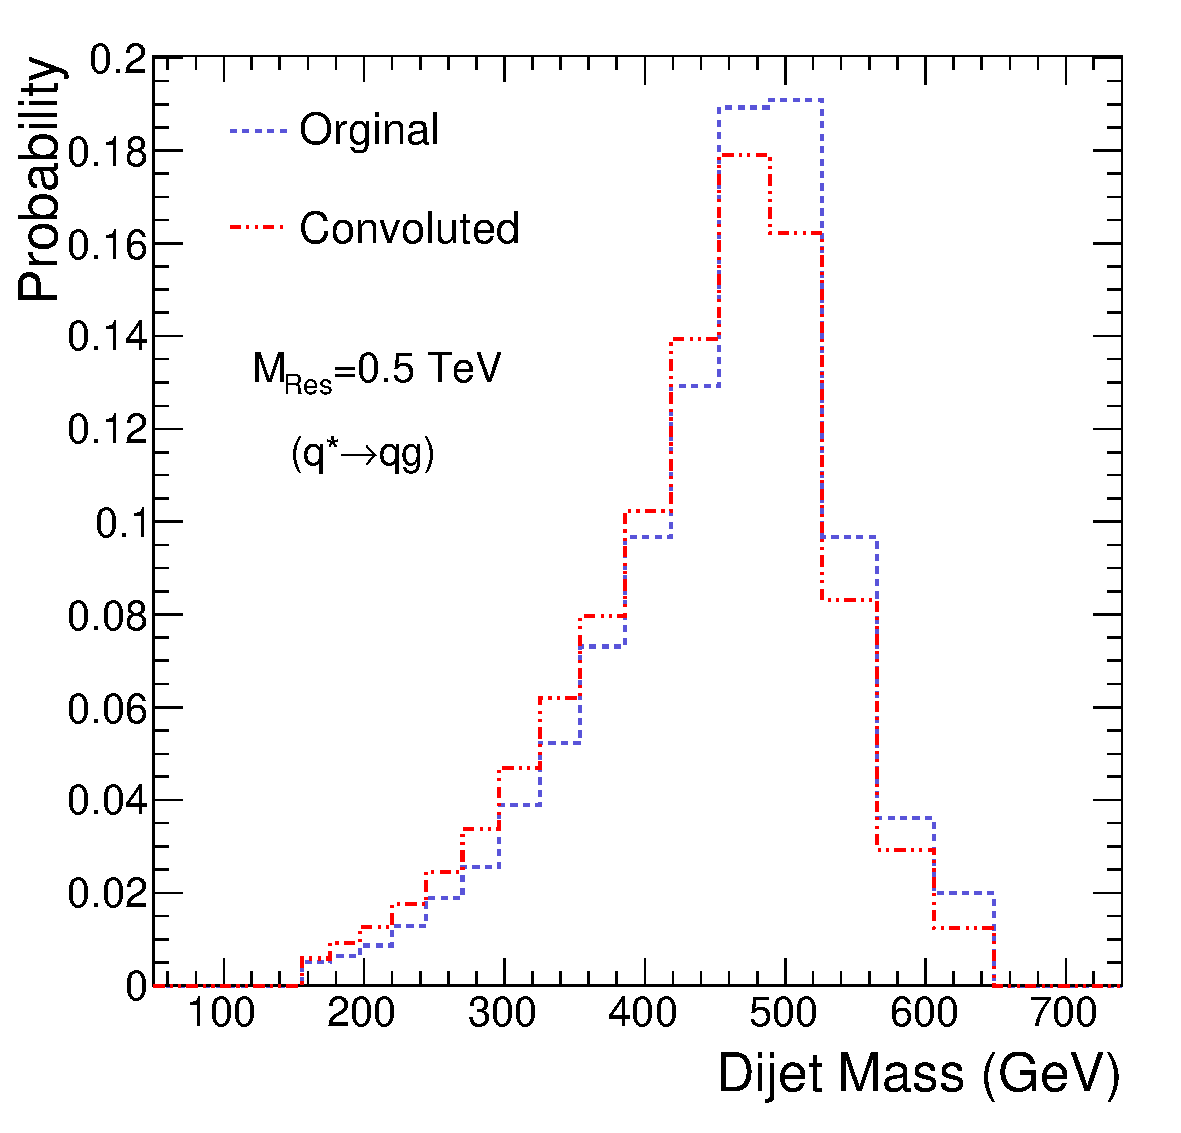
\includegraphics[width=0.3\textwidth]{Figures/Resonace_Shape_Convoluted_qg_1200.pdf}
        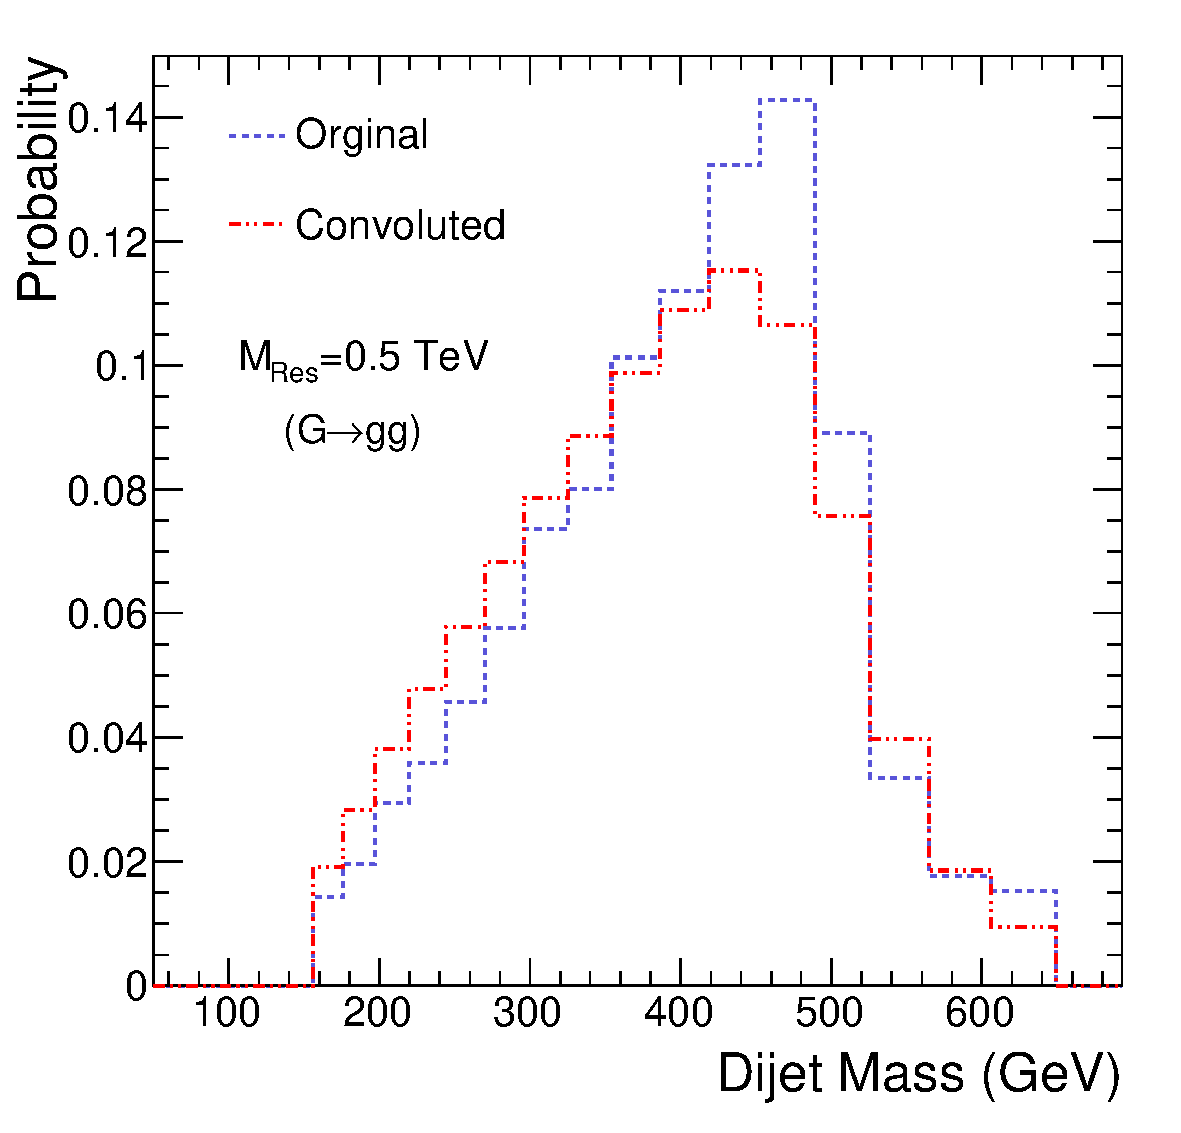
\includegraphics[width=0.3\textwidth]{Figures/Resonace_Shape_Convoluted_gg_1200.pdf}
         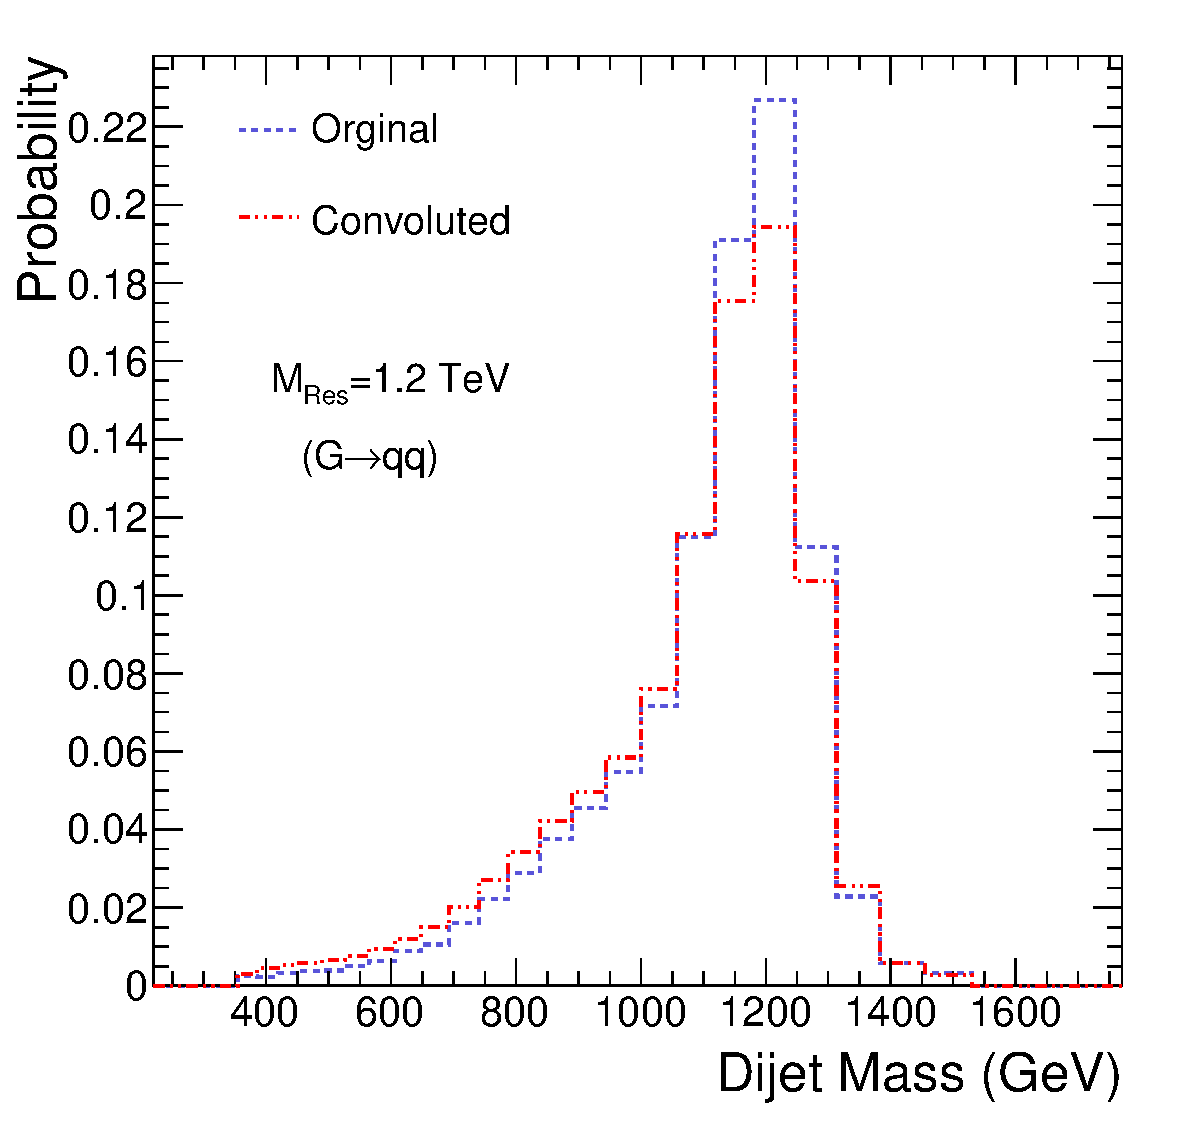
\includegraphics[width=0.3\textwidth]{Figures/Resonace_Shape_Convoluted_qq_1200_2.pdf}
          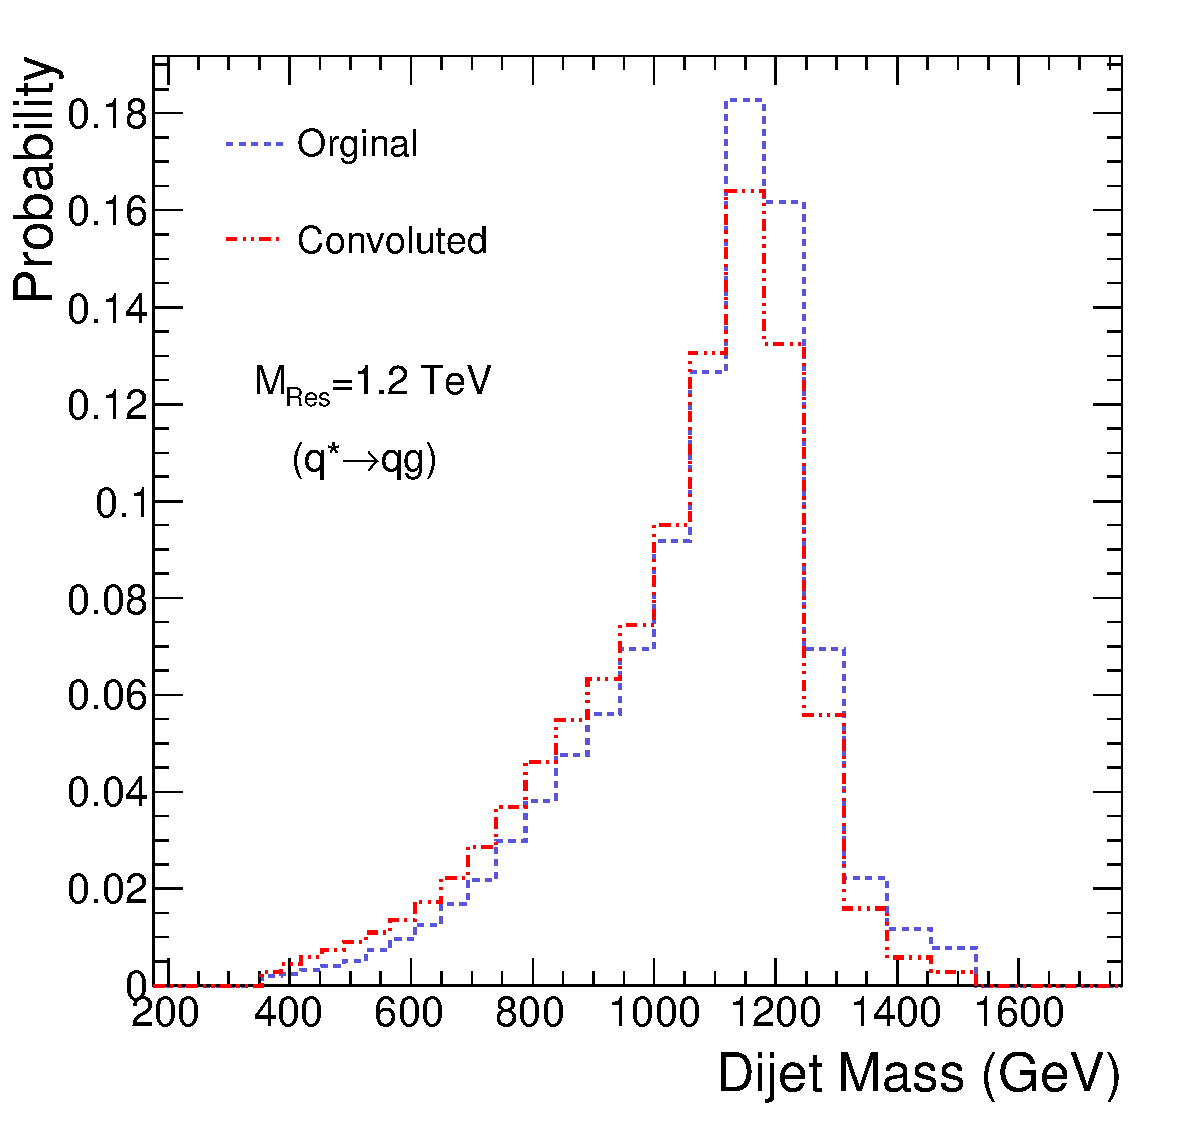
\includegraphics[width=0.3\textwidth]{Figures/Resonace_Shape_Convoluted_qg_1200_2.pdf}
           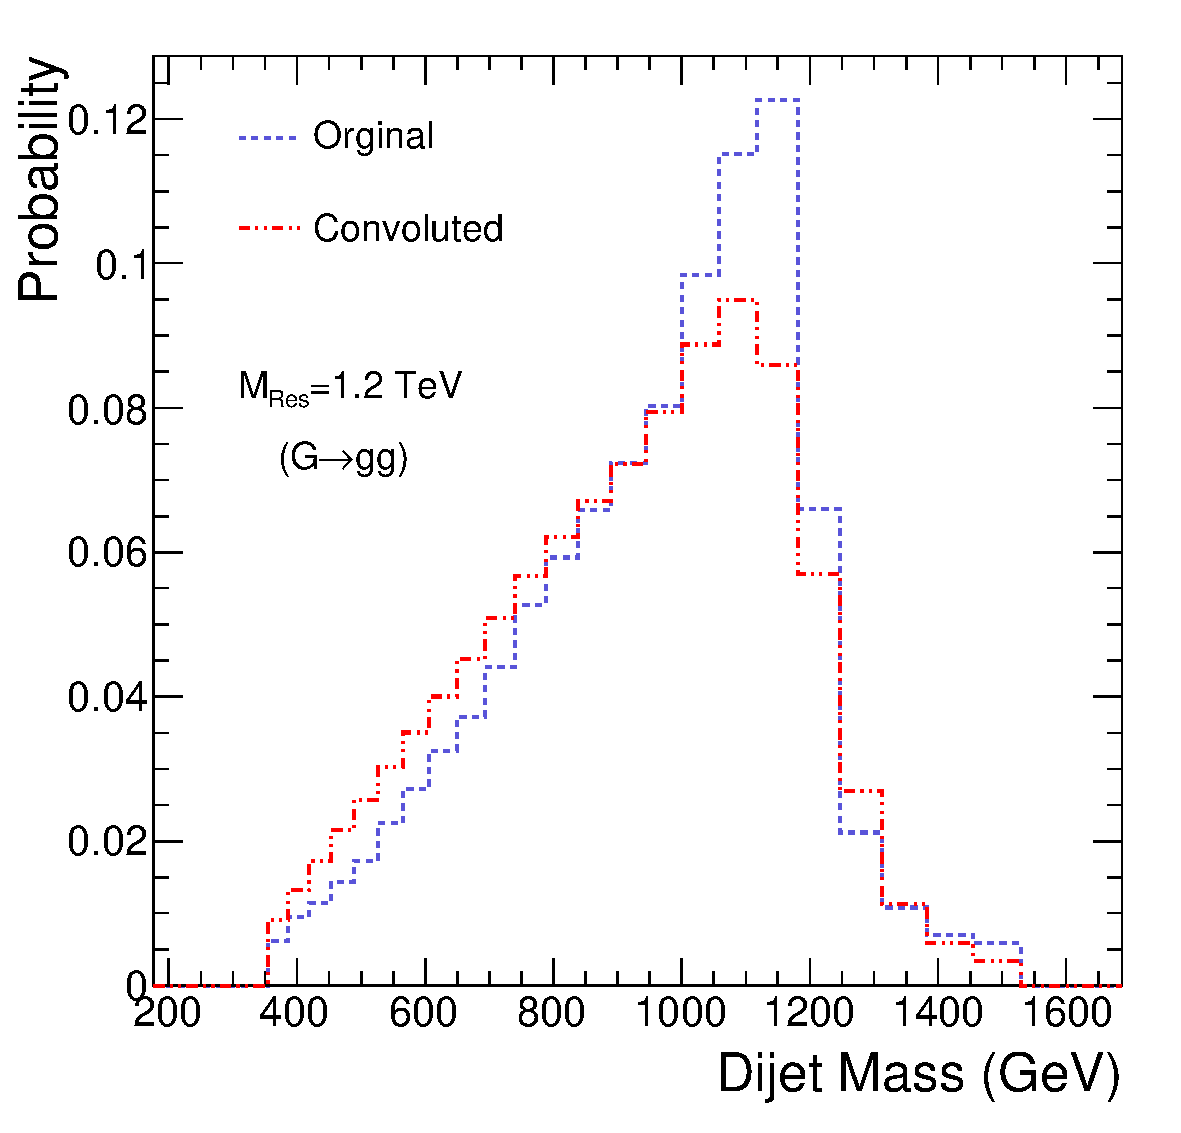
\includegraphics[width=0.3\textwidth]{Figures/Resonace_Shape_Convoluted_gg_1200_2.pdf}
    \caption{Resonance shape comparison after convolution at $0.5$ GeV (top) and $1.2$ TeV (bottom).}
    \label{conv_shape}
  \end{center}
\end{figure} 

Dijet mass core resolution of the resonance signal as a function of resonance
mass was illustrated in Fig.~\ref{resolution}. The resolution is calculated as 
$Sigma/Mean$ which are obtained from Gaussian fit of dijet mass distribution.
The fractional change on Limit with JER systematic is illustrated 
in Fig.~\ref{JER}. Effect of resolution uncertainty on limit is small.

\begin{figure}[!ht]
  \begin{center}
    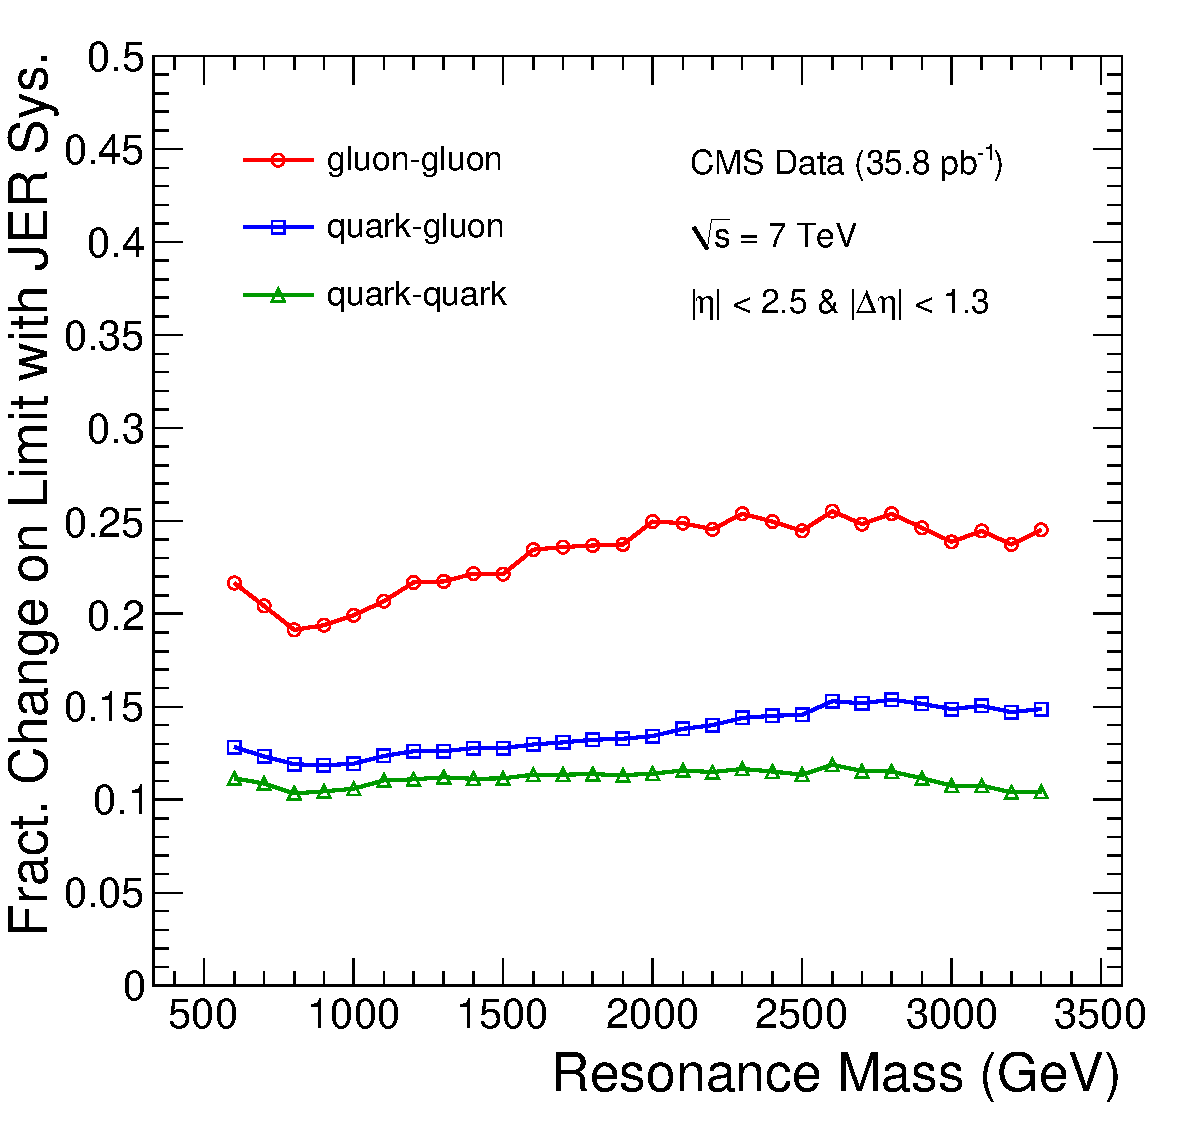
\includegraphics[width=0.6\textwidth]{Figures/Fractional_Change_JER_All.pdf}
    \caption{Fractional change on limit with JER systematic uncertainty.}
    \label{JER}
  \end{center}
\end{figure}

\clearpage


\subsection{Background Parameterization}
We considered others functional forms to parametrize the QCD background as discussed in section~\ref{sectionParam}. 
%The only form that is a good fit to our data is Alternate Fit A with 4 parameters.
We have determined the affect on the limit, for a smoothed data sample, of changing 
from our default fit to Alternate Fit A with 4 parameters.  The smooth positive envelope of the 
fractional difference is shown in Fig.~\ref{Background}.  The shallow peaking of the systematic 
is because the systematic shift is small at very low resonance mass where there are lots of events
to constrain the background and give a good fit. Then, as the resonance mass increases, the fit is more
poorly contrained by fewer events and the systematic increases. Finally. at the highest resonance 
masses there is no background, and the systematic must decrease again.
%As a result, 
%the systematic peaks at a resonance mass close to the edge of our data where there is background, but
%the background is poorly constrained by the few number of events expected. 

\begin{figure}[!ht]
  \begin{center}
%     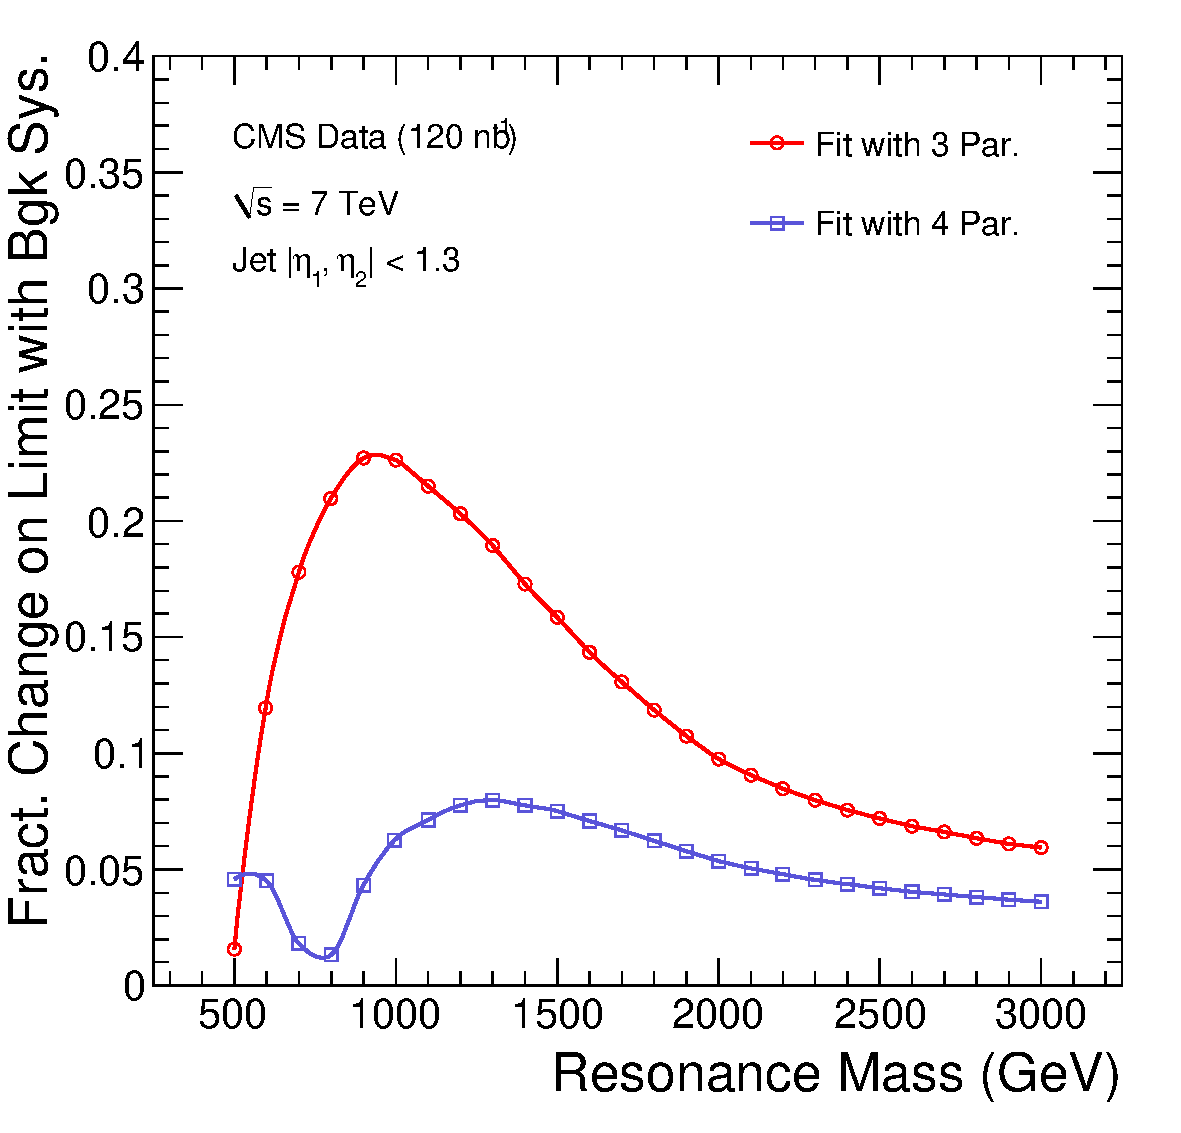
\includegraphics[width=0.45\textwidth]{Figures/Fractional_Change_Background_comparison.pdf}
       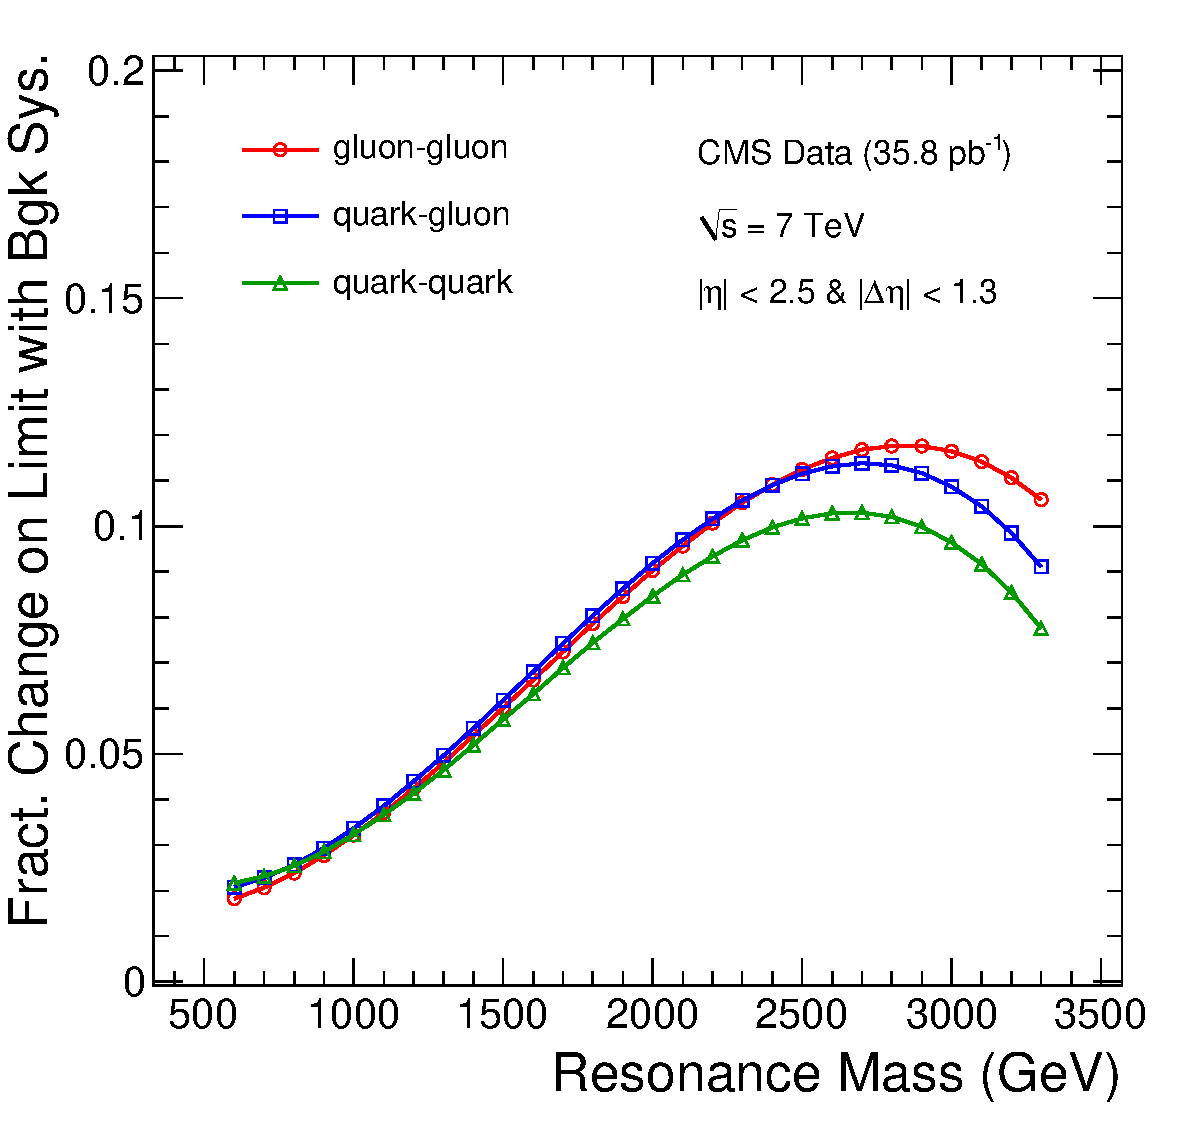
\includegraphics[width=0.6\textwidth]{Figures/Fractional_Change_Background_All.pdf}
    \caption{ Fractional change in the limit for the three resonance types when finding the background 
     using an alternate fit function.}
    \label{Background}
  \end{center}
\end{figure}

\subsection{Total Uncertainty}
We determine $1\sigma $ change for each systematic uncertainty in signal that we can discover or exclude. In
addition to the sources already mentioned, we include an uncertainty of 11\%.

To find total 
systematics, we add these $1\sigma $ changes in quadrature. 
The individual and total systematic uncertainties 
as a function 
of resonance mass are shown in Fig.~\ref{uncer}. 
Absolute uncertainty in each resonance mass is calculated as 
total fractional systematic 
uncertainty multiplied by upper cross section limit. 

\begin{figure}[!h]
  \begin{center}
         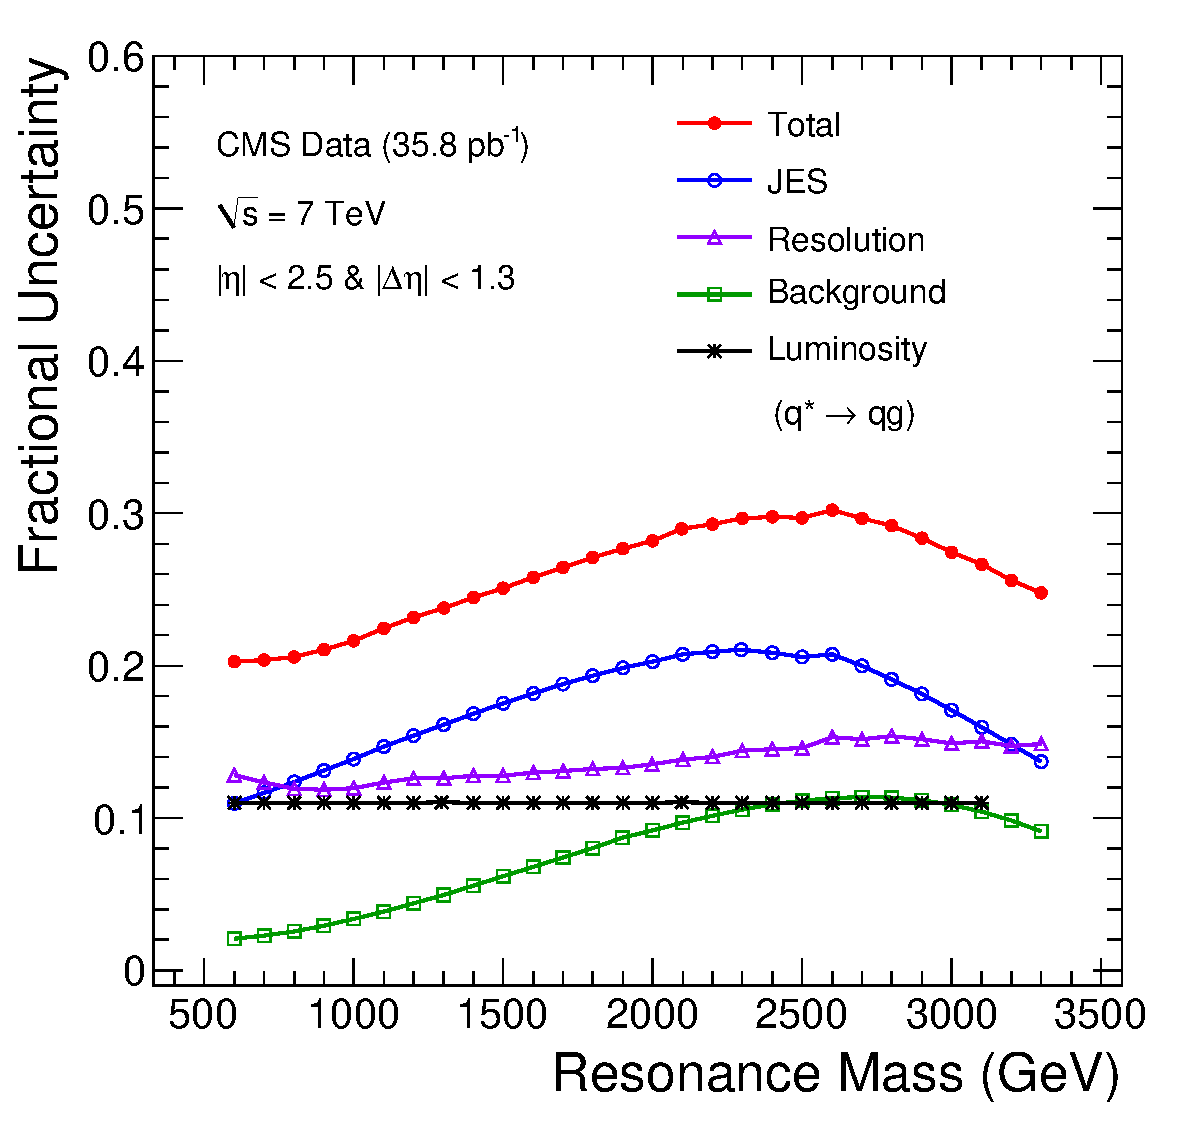
\includegraphics[width=0.45\textwidth]{Figures/Fractional_Uncer.pdf}
     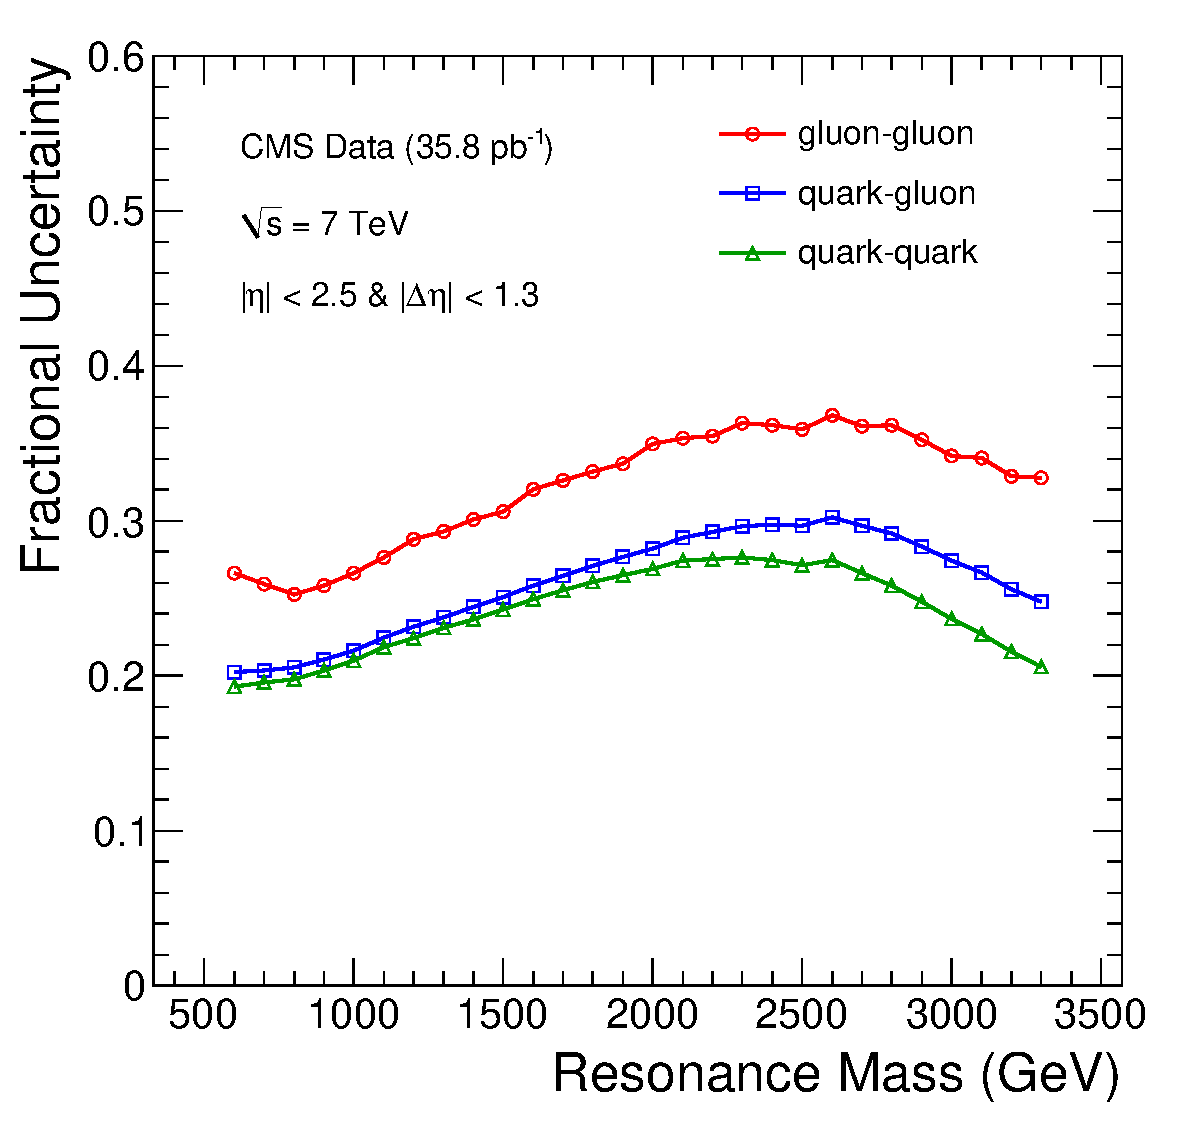
\includegraphics[width=0.45\textwidth]{Figures/Fract_Uncer_All.pdf}
    \caption{ Fractional systematic uncertainties on resonance cross section.
    Left) Individual uncertainties are shown along with the total for $qg$ resonances.
    Right) Total fractional uncertainties are compared for $qq$, $qg$, and
    $gg$ resonances.}
    \label{uncer}
  \end{center}
\end{figure}


\subsection{Incorporating Systematics in the Limit}

We convolute the posterior probability density with a Gaussian for each resonance mass. The equation of convolution is 

\begin{equation}
P_{POST}(\sigma) = \int_{0}^{\infty} P_{POST}(\sigma^{\prime}) G(\sigma, \sigma^{\prime}) d\sigma^{\prime}
\label{eqConvolution}
\end{equation}

Where $P_{POST}(\sigma^{\prime})$ is the posterior probability density at signal cross section $\sigma^{\prime}$,
and  $G(\sigma, \sigma^{\prime})$ is the Gaussian probability from systematics to observe $\sigma$ if 
$\sigma^{\prime}$ is expected.  The width of the Gaussian is taken as 
the absolute uncertainty in each resonance mass, equal to the fractional uncertainty times the limit on the cross section. This
procedure, identical to what was done at CDF in run 1~\cite{Abe:1997hm}, 
This procedure was used in CDF Run I, but has since been superseded
in CDF Run II by a more appropriate Bayesian treatment of systematics,
implemented using some formalism described in Ref~\cite{CDF5305}. 
Our procedure conservatively assigns the same width to the Gaussian in units of pb at each point 
in the posterior probability density as a function of cross section.  This produces more smearing of the probability to higher
values of cross section than using a fractional uncertainty, which would give smaller Gaussian widths at lower cross section values,
and we think it better characterizes the overall uncertainty. The convoluted value $P_{POST}(\sigma)$ is normalized
to unit area over the range $0<\sigma<\infty$.
Posterior probability densities with systematic uncertainties are shown in Appendix~\ref{appLike}. 
Total posterior probability desnity including systematics is broader and gives a higher upper limit.


For most cases, where the posterior probability density including statistical uncertainties only 
peaks at cross section values of zero, the procedure used for convolution pushes the 
probability density away from zero, creating a peak in the probability at small cross section values 
after systematics that was not there before systematics.
This does not reflect more probability for a resonance at this cross section than zero
cross section, but rather is an artifact of the convolution procedure. The procedure assigns an appreciable 
absolute systematic even at zero cross section and does not permit smearing from unphysical 
negative cross section to positive cross section, which reduces the probability for zero cross section.
This may be an artifact of using Eq.~\ref{eqConvolution} to incorporate systematics instead of a fully 
Bayesian calculation.
Caution must be used in interpreting bumps in this probability density after systematics if they
were not present and significant before systematics.  
On the contrary, for a genuine resonance, which has
significant separation from zero cross section in the posterior probability density before systematics, 
the mean value of the cross section after systematics remains the same.


 We have checked that this procedure for incorporating systematics gives reasonable results compared 
with a method used by CDF in run II~\cite{Aaltonen:2008dn}.  We have been informed that the CDF 
run II method is closer to a true Bayesian incorporation of sytematic uncertainties than the 
method we used.  The CDF run II method gives roughly 
10\% lower cross section upper limits at all resonances masses after incorporating systematics than
the method we used. We conclude that the method we used is conservative.


Our 95\% CL upper limit with statistical uncertainties only and including stystematic 
uncertainties are shown separately in Fig.~\ref{limit_change} for qg resonances. 
The effects of systematics 
on the limit is also presented in Fig.~\ref{limit_change} as a fractional change in the limit for
all three resonance types.
We note that for both string resonances and excited quarks, the mass limits are reduced by only
0.1 TeV by including systematics.
%We note that at a resonance mass of 1.7 TeV the cross section upper limit increases by
%18\% after incorporating our conservative systematic uncertainties.
%This decreases the mass limit on string resonances by only 3\%, or $0.05$ TeV.
%The effect of systematics on our string resonance mass limit is small.

\begin{figure}[!ht]
  \begin{center}
     \includegraphics[width=0.48\textwidth]{Figures/Limit_Comparison_Systematic.pdf}
    \includegraphics[width=0.48\textwidth]{Figures/Fractional_Change_Limit_All.pdf}
    \caption{Left) Limits on qg resonances with and without all systematic uncertainties. 
    Right) Fractional change in the limit after including systematics.}
    \label{limit_change}
  \end{center}
\end{figure}

\clearpage

%\begin{figure}[!ht]
%  \begin{center}
%    \includegraphics[width=0.7\textwidth]{Figures/Limit_Comparison_Systematic.pdf}
%    \caption{Comparison of 95\% cross section limits with excited quark cross section. }
%    \label{limit_change}
%  \end{center}
%\end{figure}

%\vspace*{1.5cm}
%\begin{table}[htbH]
%\centering
%\large
%\begin{tabular}{|c|c|c|}\hline
%Mass   &  \multicolumn{2}{c|}{95\% C.L. $\sigma\cdot B$ (pb)}\\
% ($TeV$) &  Stat. Error Only & Including Systematic Uncer.\\ \hline
% 0.5     &  2402             & 3915   \\
% 0.6     &  1416             & 2333   \\
% 0.7     &  1254             & 2061   \\
% 0.8     &  1101             & 1620   \\
% 0.9     &   923             & 1281   \\
% 1.0     &   746             &  953   \\
% 1.1     &   654             &  797   \\
% 1.2     &   584             &  675   \\
% 1.3     &   542             &  610   \\
% 1.4     &   507             &  562   \\
% 1.5     &   481             &  522   \\
%\hline
%\end{tabular}
%\caption{As a function of excited quark mass we list our 95\% C.L. upper limit on
%cross section times branching ratio for narrow resonances of excited quark decaying to dijets}
%\end{table}



